%Graph Spannung

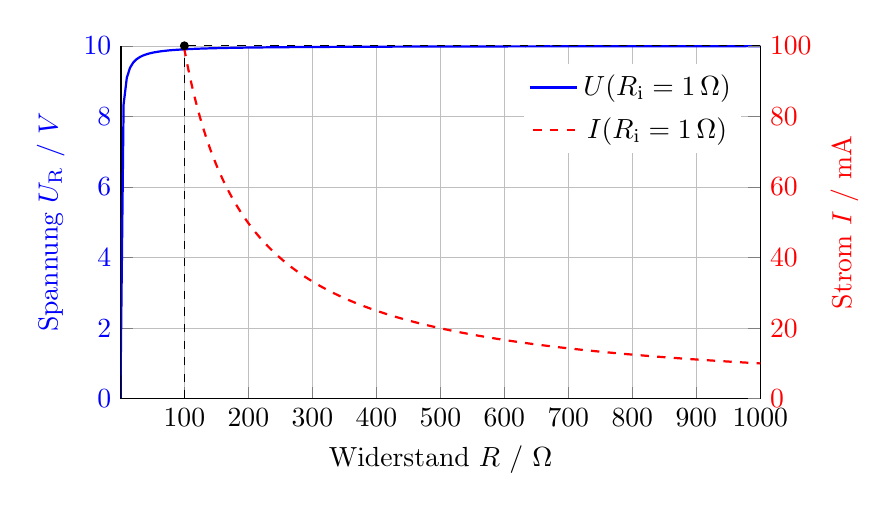
\begin{tikzpicture}
    % --- Linke Achse: Spannung ---
    \begin{axis}[
            xticklabel style={/pgf/number format/1000 sep=},
            xlabel={Widerstand $R$ / $\Omega$},
            ylabel={Spannung $U_\mathrm{R}$ / $V$},
            y label style={color=blue},
            y tick label style={color=blue},
            xmin=1, xmax=1000,
            ymin=0, ymax=10,
            xtick={0,100,...,1000},
            ytick={0,2,...,10},
            grid=both,
            major grid style={line width=.2pt,draw=gray!50},
            minor grid style={line width=.1pt,draw=gray!20},
            width=0.8\textwidth,
            height=0.5\textwidth,
            axis y line*=left,
            axis x line*=bottom,
            scaled y ticks=false,
            domain=0:1000,
            samples=200,
            legend style={
                    at={(0.80,0.95)},      % Position der Legende (x,y)(unterhalb)
                    anchor=north,          % Bezugspunkt
                    legend columns=1,      % <-- EINSPALTIG = untereinander
                    draw=none              % kein Rahmen (optional)
                }
        ]
        % Spannung
        \addplot[color=blue, thick]{10/(1+x)*x};
        \addlegendentry{$U(R_\mathrm{i}=1\,\Omega)$}
        % Strom (zweite Achse, andere Skala)
    \end{axis}

    \begin{axis}[
            ylabel={Strom $I$ / mA},
            y label style={color=red},
            y tick label style={color=red},
            xmin=1, xmax=1000,
            ymin=0, ymax=100,
            ytick={0,20,...,100},
            axis y line*=right,
            axis x line=none,
            width=0.8\textwidth,
            height=0.5\textwidth,
            scaled y ticks=false,
            legend style={
                    at={(0.80,0.83)},      % Position der Legende (unterhalb)
                    anchor=north,          % Bezugspunkt
                    legend columns=1,      % <-- EINSPALTIG = untereinander
                    draw=none              % kein Rahmen (optional)
                }
        ]
        \addplot[red, thick, dashed, domain=0:1000, samples=200]{10/(1+x)*1e3}; % in mA
        \addlegendentry{$I(R_\mathrm{i}=1\,\Omega)$}
        \only<2->{
            \draw[dashed] (axis cs:100,0)--(axis cs:100,100);
            \draw[dashed] (axis cs:1000,100)--(axis cs:100,100);
            \addplot[
                only marks,
                mark=*,
                mark options={scale=0.7, fill=black}
            ]  coordinates {
                    (100, 100)

                };


        }
    \end{axis}

\end{tikzpicture}


